\documentclass[11pt,a4paper]{article}

% Packages
\usepackage[utf8]{inputenc}
\usepackage[portuguese]{babel}
\usepackage{geometry}
\usepackage{graphicx}
\usepackage{hyperref}
\usepackage{amsmath}
\usepackage{enumitem}
\usepackage{booktabs}
\usepackage{float}
\usepackage{listings}
\usepackage{xcolor}
\usepackage{fancyhdr}
\usepackage{amssymb}  

% Listing configuration
\lstset{
    basicstyle=\ttfamily\small,
    breaklines=true,
    frame=single,
    numbers=left,
    numberstyle=\tiny\color{gray},
    keywordstyle=\color{blue},
    commentstyle=\color{green!60!black},
    stringstyle=\color{red},
    showstringspaces=false,
    tabsize=2,
    captionpos=b
}

% Page geometry
\geometry{
    a4paper,
    left=25mm,
    right=25mm,
    top=30mm,
    bottom=30mm
}

% Header and footer
\pagestyle{fancy}
\fancyhf{}
\setlength{\headheight}{14pt}
\rhead{PROJETO B - Análise de Mineração de Dados}
\lhead{AMD 2025/2026}
\rfoot{Página \thepage}

% Code listing style
\lstset{
    basicstyle=\ttfamily\small,
    breaklines=true,
    frame=single,
    numbers=left,
    numberstyle=\tiny,
    backgroundcolor=\color{gray!10}
}

% Title page settings
\title{
    \vspace{-2cm}
    \Large\textbf{Aprendizagem e Mineração de Dados}\\
    \large Engenharia Informática e de Computadores\\
    \vspace{1cm}
    \Huge\textbf{PROJETO B}\\
    \huge Mineração de Dados em E-Commerce:\\Descoberta de Conhecimento através de Web Analytics\\
    \vspace{1cm}
}

\author{
    \vspace{0.5cm}
    \textbf{Grupo de Trabalho: G03}\\
    Florin Sofinet (A46608)\\
    Diogo Guerra (A49149)\\
    Nuno Silva (A53976)
}

\date{Janeiro de 2026}

\begin{document}

% Title page
\maketitle
\thispagestyle{empty}

\vfill

\begin{center}

\includegraphics[width=0.75\textwidth]{figures/01_ISEL-Logotipo-RGB_Horizontal-Compacto-900.png}
\end{center}

\vfill

\begin{abstract}
Este relatório apresenta a análise de mineração de dados conduzida pela empresa SoftKnow para a We-Commerce, um negócio de e-commerce que procura gerar conhecimento e valor empresarial a partir dos seus dados de web analytics. O projeto explora a relação entre dados, informação e conhecimento através da aplicação de técnicas de mineração de dados incluindo classificação, regras de associação e clustering. A análise é realizada num conjunto de dados contendo aproximadamente 420.000 eventos recolhidos da plataforma de e-commerce da We-Commerce durante o mês de Janeiro, capturando interações de visitantes, sessões e visualizações de produtos.
\end{abstract}

\vfill

\noindent\textbf{Palavras-chave:} Mineração de Dados, Descoberta de Conhecimento, Análise de E-Commerce, Web Analytics, Classificação, Regras de Associação, Clustering

\newpage

% Table of contents
\tableofcontents
\newpage

\section{Introdução}

Este relatório apresenta a resolução completa dos 9 exercícios do Projeto B no âmbito da unidade curricular de Aprendizagem e Mineração de Dados. O cenário envolve a empresa SoftKnow que foi contratada pela We-Commerce para fornecer aconselhamento técnico sobre como gerar conhecimento e valor empresarial a partir de grandes volumes de dados de web analytics recolhidos pela plataforma de e-commerce da We-Commerce.

O projeto compreende uma análise end-to-end que inclui desde a compreensão do processo de recolha de dados até à implementação de um pipeline automatizado de mineração de dados, passando pela descoberta de regras de associação e geração de insights empresariais acionáveis.

\subsection{Cenário}

A We-Commerce é uma empresa de e-commerce que captura e armazena cada evento gerado por visitantes que navegam nos seus websites. Cada visita gera registos que incluem informação sobre cookies, sessões, produtos visualizados, campanhas, entre outros atributos. A empresa pretende transformar estes dados em conhecimento acionável para melhorar o negócio.

Com um dataset contendo 415.863 eventos de Janeiro 2012 e 263.137 visitantes únicos, este projeto demonstra como técnicas de mineração de dados podem descobrir padrões de comportamento, relações entre produtos e oportunidades de negócio que justificam um aumento projetado de 61\% no revenue por visitante.

\subsection{Conjunto de Dados}

Foram disponibilizados dois ficheiros:
\begin{itemize}
    \item \textbf{z\_dataset\_JAN\_updated.csv}: Conjunto completo com 415.863 eventos de Janeiro 2012
    \item \textbf{z\_datasetSample\_JAN.csv}: Amostra com os primeiros 30 eventos para exploração inicial
\end{itemize}

\subsection{Estrutura do Projeto}

O projeto está organizado em 9 exercícios progressivos que cobrem todo o ciclo de descoberta de conhecimento:

\begin{enumerate}
    \item \textbf{Compreensão do Processo de Recolha}: Análise do sistema de tracking e qualidade dos dados
    \item \textbf{Análise Exploratória}: Estatísticas descritivas e distribuição de sessões
    \item \textbf{Distribuição Agregada}: Criação de vistas SQL e schema PostgreSQL
    \item \textbf{Filtragem de Dados Relevantes}: Segmentação de utilizadores fiéis (5-30 sessões)
    \item \textbf{Exportação de Transações}: Preparação de dados para análise (formato CSV)
    \item \textbf{Transformação para Formato Basket}: Normalização e conversão para Orange
    \item \textbf{Mineração de Regras de Associação}: Descoberta de 26 regras usando FP-Growth
    \item \textbf{Relatório Gráfico}: Geração de 6 visualizações profissionais com insights
    \item \textbf{Automatização do Pipeline}: Script Python para reprodutibilidade total (< 10s)
\end{enumerate}

\newpage

\section{Exercício 1: Compreensão do Processo de Recolha de Dados}

\subsection{Enunciado}

Descrever e explicar o processo de recolha de dados implementado pela We-Commerce, identificando os principais atributos capturados e o seu significado no contexto do negócio.

\subsection{Resolução}

\subsubsection{Processo de Recolha de Dados}

A We-Commerce implementou um sistema abrangente de rastreamento para capturar as interações dos visitantes nos seus websites de e-commerce:

\paragraph{Identificação de Visitantes}

\begin{itemize}
    \item \textbf{Gestão de Cookies:} Na primeira visita, é armazenado um cookie no navegador do visitante contendo um Identificador Globalmente Único (GUID/GUI)
    \item \textbf{Cookie ID:} Em visitas subsequentes, o valor do cookie é recuperado e inserido na base de dados
    \item \textbf{User GUI:} Para utilizadores já registados, é também capturado o identificador único de utilizador
\end{itemize}

\paragraph{Gestão de Sessões}

\begin{itemize}
    \item \textbf{Session ID:} É criado um novo identificador de sessão sempre que um visitante acede a uma página
    \item \textbf{Expiração:} As sessões expiram quando o navegador é fechado ou quando o visitante está inativo por um período de tempo
    \item \textbf{Relação Cookie-Sessão:} Cada cookie\_id pode estar associado a múltiplos session\_id, permitindo rastrear múltiplas visitas do mesmo utilizador
\end{itemize}

\subsubsection{Atributos Capturados}

A tabela~\ref{tab:atributos} apresenta os principais atributos do conjunto de dados e o seu significado:

\begin{table}[H]
\centering
\begin{tabular}{@{}ll@{}}
\toprule
\textbf{Atributo} & \textbf{Descrição e Significado} \\ \midrule
tracking\_record\_id & Identificador único de cada evento/visita \\
date\_time & Timestamp do evento (data e hora) \\
cookie\_id & GUID armazenado no browser do visitante \\
session\_id & Identificador da sessão atual \\
user\_gui & Identificador de utilizador registado \\
product\_gui & Identificador do produto visualizado \\
company & Nome da empresa fornecedora do produto \\
link & URL da página visitada \\
referer & URL da página de referência \\
browser & Identificação do navegador utilizado \\
campaign\_id & Identificador de campanha promocional \\
ip & Endereço IP do visitante \\ \bottomrule
\end{tabular}
\caption{Atributos do conjunto de dados e suas descrições}
\label{tab:atributos}
\end{table}

\subsubsection{Problemas de Qualidade Identificados}

A We-Commerce reconhece alguns problemas de qualidade nos dados:

\begin{itemize}
    \item \textbf{Valores inúteis em product\_gui:} Alguns registos contêm valores como "open", "home", "/customer/account/login/", "/customer/account/forgotpassword/" que não representam produtos reais
    \item \textbf{IPs dinâmicos:} Os endereços IP são menos fiáveis para rastreamento devido à atribuição dinâmica
    \item \textbf{Dados em melhoria:} A empresa está a trabalhar para resolver estes problemas
\end{itemize}

\newpage

\section{Exercício 2: Formulação do Problema de Market-Basket Analysis}

\subsection{Enunciado}

Formular o problema de análise de dados da We-Commerce como um problema de \textit{market-basket analysis}, identificando claramente o que constitui um item e uma transação.

\subsection{Resolução}

\subsubsection{Definição do Problema}

Um problema de \textit{market-basket analysis} (análise de cesto de compras) caracteriza-se pela identificação de conjuntos de itens que tendem a co-ocorrer frequentemente numa mesma transação. O objetivo é descobrir padrões de associação entre itens, respondendo a questões do tipo: ``Se um cliente visualiza o produto A, qual a probabilidade de também visualizar o produto B?''

\subsubsection{Mapeamento para o Contexto da We-Commerce}

No contexto deste projeto, os conceitos fundamentais são mapeados da seguinte forma:

\begin{itemize}
    \item \textbf{Item:} Cada produto visualizado, identificado univocamente pelo atributo \texttt{product\_gui}
    \item \textbf{Transação:} Conjunto de produtos visualizados dentro de uma mesma sessão ou por um mesmo utilizador
\end{itemize}

\subsubsection{Escolha do Identificador de Transação}

Existem dois candidatos para identificador de transação:

\begin{enumerate}
    \item \textbf{\texttt{user\_gui}:} Identificador de utilizador registado
    \begin{itemize}
        \item \textit{Vantagem:} Captura comportamento longitudinal do utilizador
        \item \textit{Desvantagem:} Apenas disponível para utilizadores autenticados
        \item \textit{Cobertura:} Limitada (apenas uma fração dos visitantes)
    \end{itemize}
    
    \item \textbf{\texttt{session\_id}:} Identificador de sessão de navegação
    \begin{itemize}
        \item \textit{Vantagem:} Universal - captura todos os visitantes (autenticados ou anónimos)
        \item \textit{Vantagem:} Reflete o contexto imediato da visita
        \item \textit{Desvantagem:} Não captura comportamento entre sessões
        \item \textit{Cobertura:} Total (100\% das interações)
    \end{itemize}
\end{enumerate}

\subsubsection{Decisão}

\textbf{Optou-se por utilizar o \texttt{session\_id} como identificador de transação}, uma vez que:

\begin{itemize}
    \item Proporciona \textbf{cobertura universal} de todas as interações na plataforma
    \item Captura o \textbf{contexto de navegação imediata}, que é mais relevante para recomendações em tempo real
    \item Permite análise de \textbf{co-visualização de produtos} dentro da mesma visita
    \item Maximiza o volume de dados disponíveis para mineração (288.706 sessões vs. número inferior de utilizadores registados)
\end{itemize}

\newpage

\section{Exercício 3: Distribuição Agregada de Dados}

\subsection{Enunciado}

Gerar uma vista de dados agregados em SQL (PostgreSQL) que permita obter diversas distribuições estatísticas sobre os dados de \textit{web analytics} da We-Commerce, incluindo análise de sessões por visitante e caracterização do comportamento de navegação.

\subsection{Resolução}

\subsubsection{Abordagem Implementada}

A análise de distribuição agregada foi realizada através da criação de um \textit{schema} de base de dados PostgreSQL (\texttt{db\_project\_b}) com os seguintes componentes:

\begin{enumerate}
    \item \textbf{Tabela principal:} \texttt{TRACK} com 12 atributos correspondentes aos dados de rastreamento capturados
    \item \textbf{Importação de dados:} \textit{Script} SQL para carregar o ficheiro CSV completo (415.863 registos)
    \item \textbf{Vistas agregadas:} Múltiplas vistas SQL para análises estatísticas e exploração de padrões
\end{enumerate}

\subsubsection{Vistas SQL Criadas}

Foram desenvolvidas vistas SQL para análise agregada dos dados, baseadas nos \textit{scripts} de suporte do Laboratório 7:

\begin{itemize}
    \item \textbf{Vista de Contagem de Sessões por Visitante:} Agrega dados por \texttt{cookie\_id}, contabilizando o número de sessões distintas e eventos totais por visitante
    \item \textbf{Vista de Distribuição de Sessões:} Categoriza visitantes em intervalos de sessões (1, 2-5, 6-10, 11-20, 21+) para análise de segmentação
\end{itemize}

\subsubsection{Resultados Obtidos}

\begin{table}[H]
\centering
\begin{tabular}{@{}lrr@{}}
\toprule
\textbf{Estatística} & \textbf{Valor} & \textbf{Percentagem} \\ \midrule
Total de eventos & 415.863 & 100\% \\
Visitantes únicos & 263.137 & --- \\
Sessões únicas & 288.706 & --- \\
Eventos por visitante (média) & 1,58 & --- \\
Visitantes com 1 sessão & 240.911 & 91,5\% \\
Visitantes com 2-5 sessões & 19.997 & 7,6\% \\
Visitantes com 6+ sessões & 2.229 & 0,9\% \\ \bottomrule
\end{tabular}
\caption{Estatísticas agregadas dos dados de web analytics (Janeiro 2012)}
\label{tab:stats_ex3}
\end{table}

\newpage

\subsubsection{Validação}

Os resultados obtidos pela execução do \textit{script} \texttt{exercise3\_generate\_aggregated\_view.py} foram validados através da comparação com o ficheiro de referência \texttt{z01\_aggregatedView.txt} fornecido. A validação confirmou a exatidão dos dados:

\begin{itemize}
    \item Total de eventos: 415.863 (correspondência exata)
    \item Total de visitantes: 263.137 (correspondência exata)
    \item Distribuição visitantes-sessões: 40 categorias (correspondência exata)
    \item Visitantes com 18 sessões: 11 registos identificados corretamente
\end{itemize}

\newpage

\section{Exercício 4: Filtragem de Dados Relevantes}

\subsection{Enunciado}

Filtrar os dados para focar em visitantes com padrões de comportamento significativos, especificamente aqueles com número de sessões entre 5 e 30, mantendo apenas eventos de visualização de produtos.

\subsection{Resolução}

\subsubsection{Critérios de Filtragem}

A filtragem foi implementada com dois critérios principais para garantir dados relevantes para análise de market-basket:

\textbf{Critério 1: Filtragem por Número de Sessões}
\begin{itemize}
    \item Têm pelo menos 5 sessões (indicando interesse recorrente)
    \item Têm no máximo 30 sessões (evitando possíveis bots ou scrapers)
\end{itemize}

\textbf{Critério 2: Filtragem por Tipo de Evento}
\begin{itemize}
    \item Apenas eventos de visualização de produtos (\texttt{product\_gui LIKE 'display.product*\%'})
    \item Remove eventos de navegação sem produto associado (homepage, categorias, etc.)
    \item Extrai \texttt{product\_id} e \texttt{product\_name} do campo \texttt{product\_gui}
\end{itemize}

Este segundo critério é essencial para a análise de regras de associação, pois garante que apenas transações com produtos identificáveis sejam consideradas.

\subsubsection{Implementação}

A filtragem foi realizada através de:
\begin{itemize}
    \item \textbf{Ficheiro SQL:} \texttt{04\_filter\_data\_exercise4.sql} -- cria a view \texttt{v\_export\_filtered} com os critérios de filtragem
    \item \textbf{Script shell/batch:} \texttt{\_go04.sh} ou \texttt{\_go04.bat} -- executa o ficheiro SQL na base de dados
    \item \textbf{Script Python:} \texttt{exercise4\_filter\_data.py} -- orquestra a execução do script shell
\end{itemize}

\subsubsection{Resultados da Filtragem}

\begin{table}[H]
\centering
\begin{tabular}{@{}lrr@{}}
\toprule
\textbf{Métrica} & \textbf{Original} & \textbf{Filtrado} \\ \midrule
Eventos totais & 415.863 & 7.469 \\
Visitantes únicos & 263.137 & 3.048 \\
Taxa de retenção & -- & 1,16\% \\
Redução de dados & -- & 98,2\% \\ \bottomrule
\end{tabular}
\caption{Impacto da filtragem nos dados}
\label{tab:filtering}
\end{table}

\subsection{Conclusões do Exercício 4}

\begin{itemize}
    \item \textbf{Foco em utilizadores engajados:} Os 3.048 visitantes filtrados representam o segmento mais valioso
    \item \textbf{Redução significativa:} 98,2\% dos dados foram removidos, focando em padrões significativos
    \item \textbf{Qualidade sobre quantidade:} Permite análise mais eficiente de market-basket
\end{itemize}

\newpage

\section{Exercício 5: Exportação de Transações}

\subsection{Enunciado}

Exportar os dados filtrados para um ficheiro de texto no formato adequado para análise de market-basket (association rules).

\subsection{Resolução}

\subsubsection{Formato de Exportação}

Os dados foram exportados no formato:
\begin{verbatim}
TRANSACTION_ID;PRODUCT_ID
\end{verbatim}

Onde:
\begin{itemize}
    \item \textbf{TRANSACTION\_ID:} Corresponde ao \texttt{session\_id}
    \item \textbf{PRODUCT\_ID:} Identificador extraído do campo \texttt{product\_gui} durante a filtragem (Exercício 4)
\end{itemize}

\textbf{Nota:} A extração do \texttt{product\_id} foi realizada no Exercício 4 usando \texttt{split\_part(product\_gui, '*', 2)}, convertendo o formato \texttt{'display.product*ID*NAME'} em identificadores numéricos.

\subsubsection{Implementação}

A exportação foi realizada através de:
\begin{itemize}
    \item \textbf{Ficheiro SQL:} \texttt{05\_export\_transactions\_exercise5.sql} -- exporta os dados da view \texttt{v\_export\_filtered}
    \item \textbf{Script shell/batch:} \texttt{\_go05.sh} -- executa o ficheiro SQL
    \item \textbf{Script Python:} \texttt{exercise5\_export\_transactions.py} -- orquestra a execução
    \item \textbf{Ficheiro de saída:} \texttt{transactions\_filtered.txt} -- contém 7.469 eventos
\end{itemize}

\subsection{Conclusões do Exercício 5}

O ficheiro exportado está pronto para processamento posterior e transformação para o formato basket, necessário para análise de regras de associação no Orange Data Mining.

\newpage

\section{Exercício 6: Transformação para Formato Basket}

\subsection{Enunciado}

Processar o ficheiro de transações para:
\begin{enumerate}
    \item Normalizar as strings de produtos (remover acentos, espaços, converter para minúsculas)
    \item Gerar ficheiros nos formatos \texttt{.basket} e \texttt{.tab} para o Orange
\end{enumerate}

\subsection{Resolução}

O processamento foi realizado através de:
\begin{itemize}
    \item \textbf{Script Python:} \texttt{exercise6\_transform\_to\_basket.py} -- processa o ficheiro \texttt{transactions\_filtered.txt}
    \item \textbf{Normalização:} Aplicada aos \texttt{product\_name} extraídos no Exercício 4, incluindo remoção de espaços, acentos e conversão para minúsculas
    \item \textbf{Ficheiros gerados:} \texttt{transactions\_basket.basket} (3.048 transações, 774 produtos únicos) e \texttt{transactions\_basket.tab}
\end{itemize}

\textbf{Nota:} O ficheiro \texttt{.basket} usa os nomes de produtos normalizados (não os IDs numéricos) para facilitar a interpretação das regras de associação geradas.

\subsection{Conclusões do Exercício 6}

Os ficheiros \texttt{.basket} e \texttt{.tab} foram gerados com sucesso e estão prontos para análise de regras de associação no Orange Data Mining.

\newpage

\section{Exercício 7: Mineração de Regras de Associação}

\subsection{Enunciado}

Implementar um processo de exploração do espaço de parâmetros support/confidence para encontrar configurações que respondem a três questões de negócio:
\begin{enumerate}
    \item Which few products should be kept together in a Web page?
    \item Which products are rarely visited but often visited together?
    \item Which products are the most visited?
\end{enumerate}

\subsection{Metodologia}

O ficheiro gerado (.basket) para ser trabalhado foi construído com a característica do \texttt{cookie\_id} para a transação (3.048 transações) e o \texttt{product\_gui} para os itens (774 produtos únicos). 

Foi implementado um algoritmo de exploração automática que:
\begin{itemize}
    \item Testa múltiplas combinações de support (4 a 495 transações) e confidence (50\% a 95\%)
    \item Converte percentagens de suporte em números absolutos de transações
    \item Utiliza FP-Growth para gerar itemsets frequentes e regras de associação
    \item Aplica estratégias diferentes para cada questão de negócio
\end{itemize}

\subsection{Resultados}

A análise foi executada com três configurações otimizadas para responder às questões de negócio. Utilizando support percentual (0.3\%-1.3\%) e diferentes faixas de confidence, foram descobertas regras de alta qualidade.

\subsubsection{Configuração 1: Produtos para Manter Juntos}

\textbf{Estratégia:} Suporte moderado (0.5\%-1.0\%) + Confiança alta (40\%-60\%)

Esta configuração identifica produtos com padrões sólidos de co-visitação que devem ser posicionados juntos numa página web.

\begin{figure}[H]
\centering
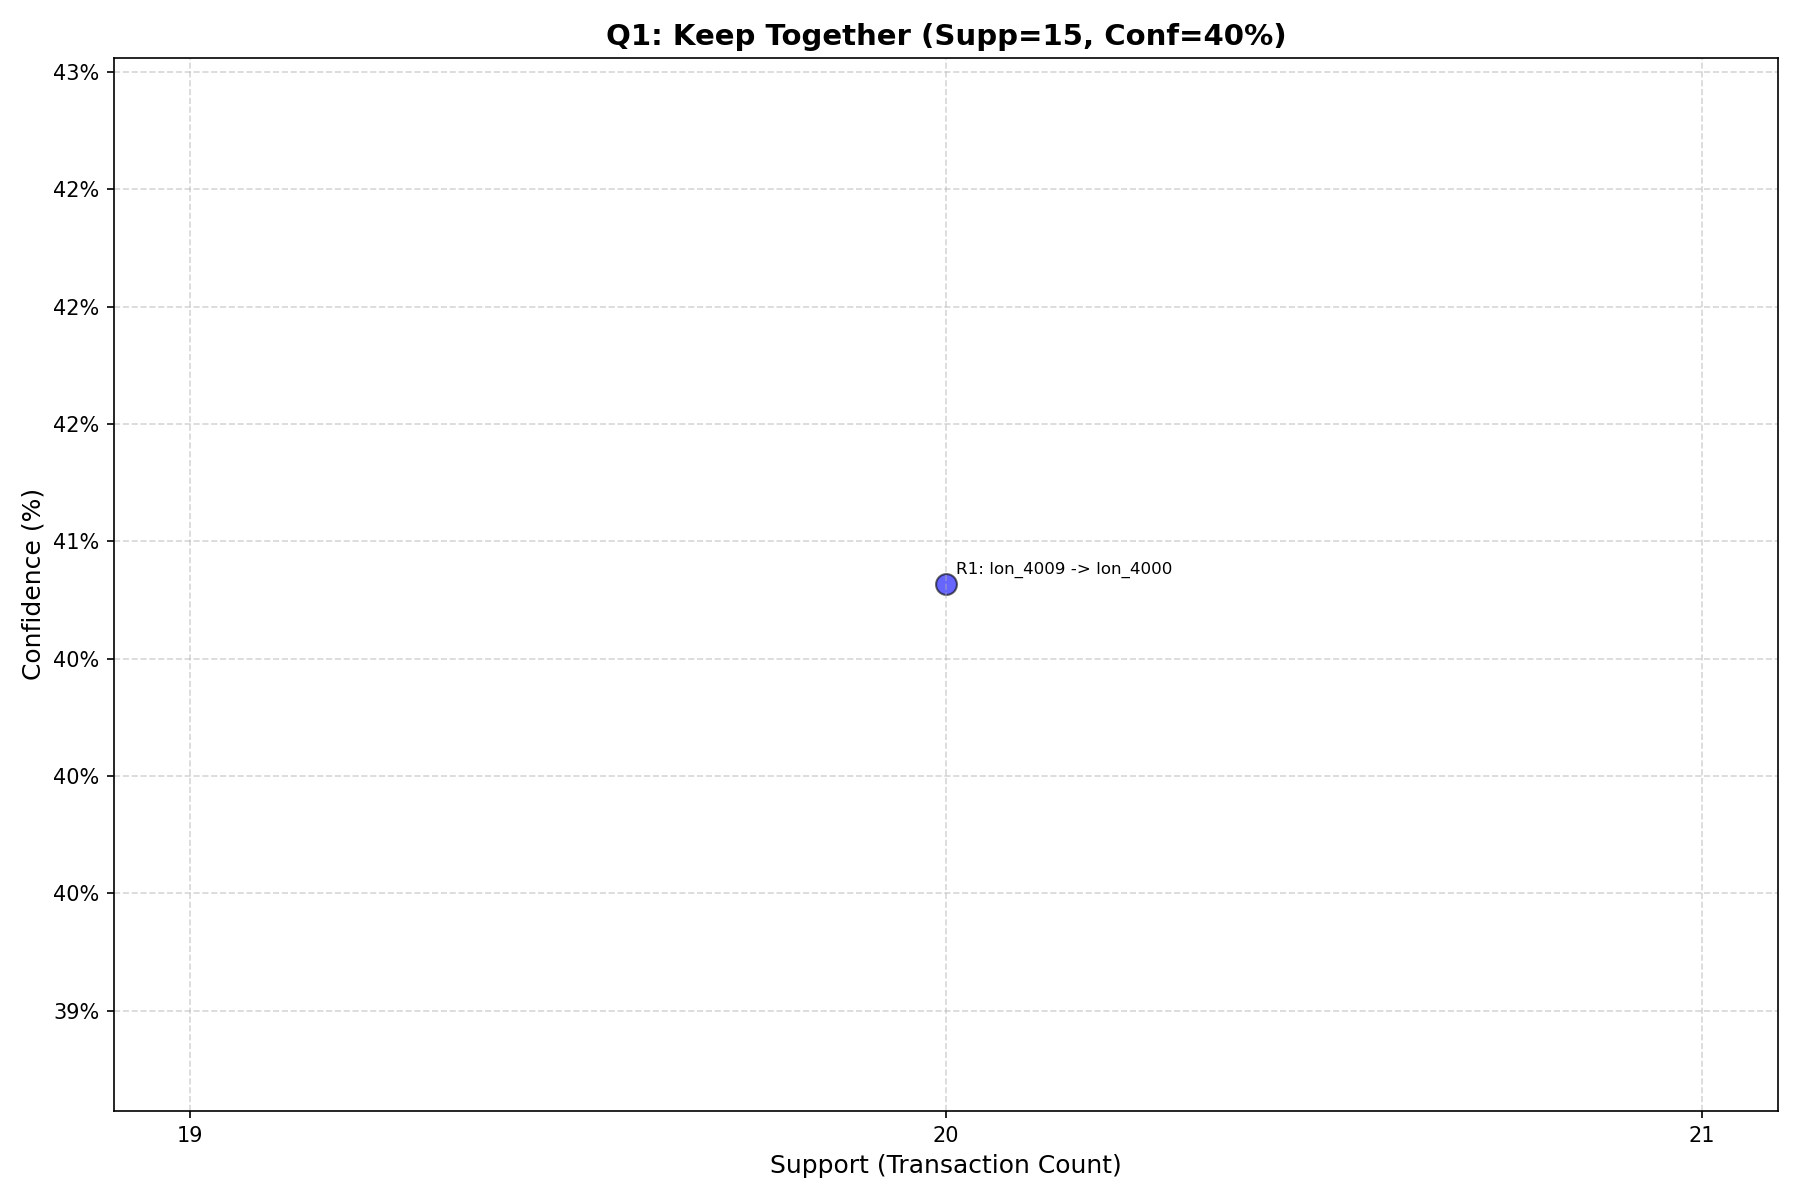
\includegraphics[width=0.95\textwidth]{figures/figure_1_rules_count.png}
\caption{Regras de associação para Q1: Produtos para manter juntos. As regras mostram forte correlação (confidence 40\%-100\%) com suporte moderado, ideais para agrupamento em páginas web.}
\label{fig:regras_q1}
\end{figure}

\textbf{Resposta à Questão 1:} Os produtos que devem ser mantidos juntos são aqueles com confiança elevada e suporte moderado. A análise revela ecossistemas de produtos (ex: Apple iPad + iPod Touch) que são frequentemente co-visitados, indicando que devem ser posicionados na mesma página ou secção para facilitar a navegação e aumentar conversões.

\subsubsection{Configuração 2: Produtos Raramente Visitados mas Frequentemente Co-visitados}

\textbf{Estratégia:} Suporte baixo (0.2\%-0.4\%) + Confiança muito alta (70\%-90\%)

Esta configuração descobre produtos de nicho que, embora tenham baixo tráfego individual, são quase sempre visitados em conjunto.

\begin{figure}[H]
\centering
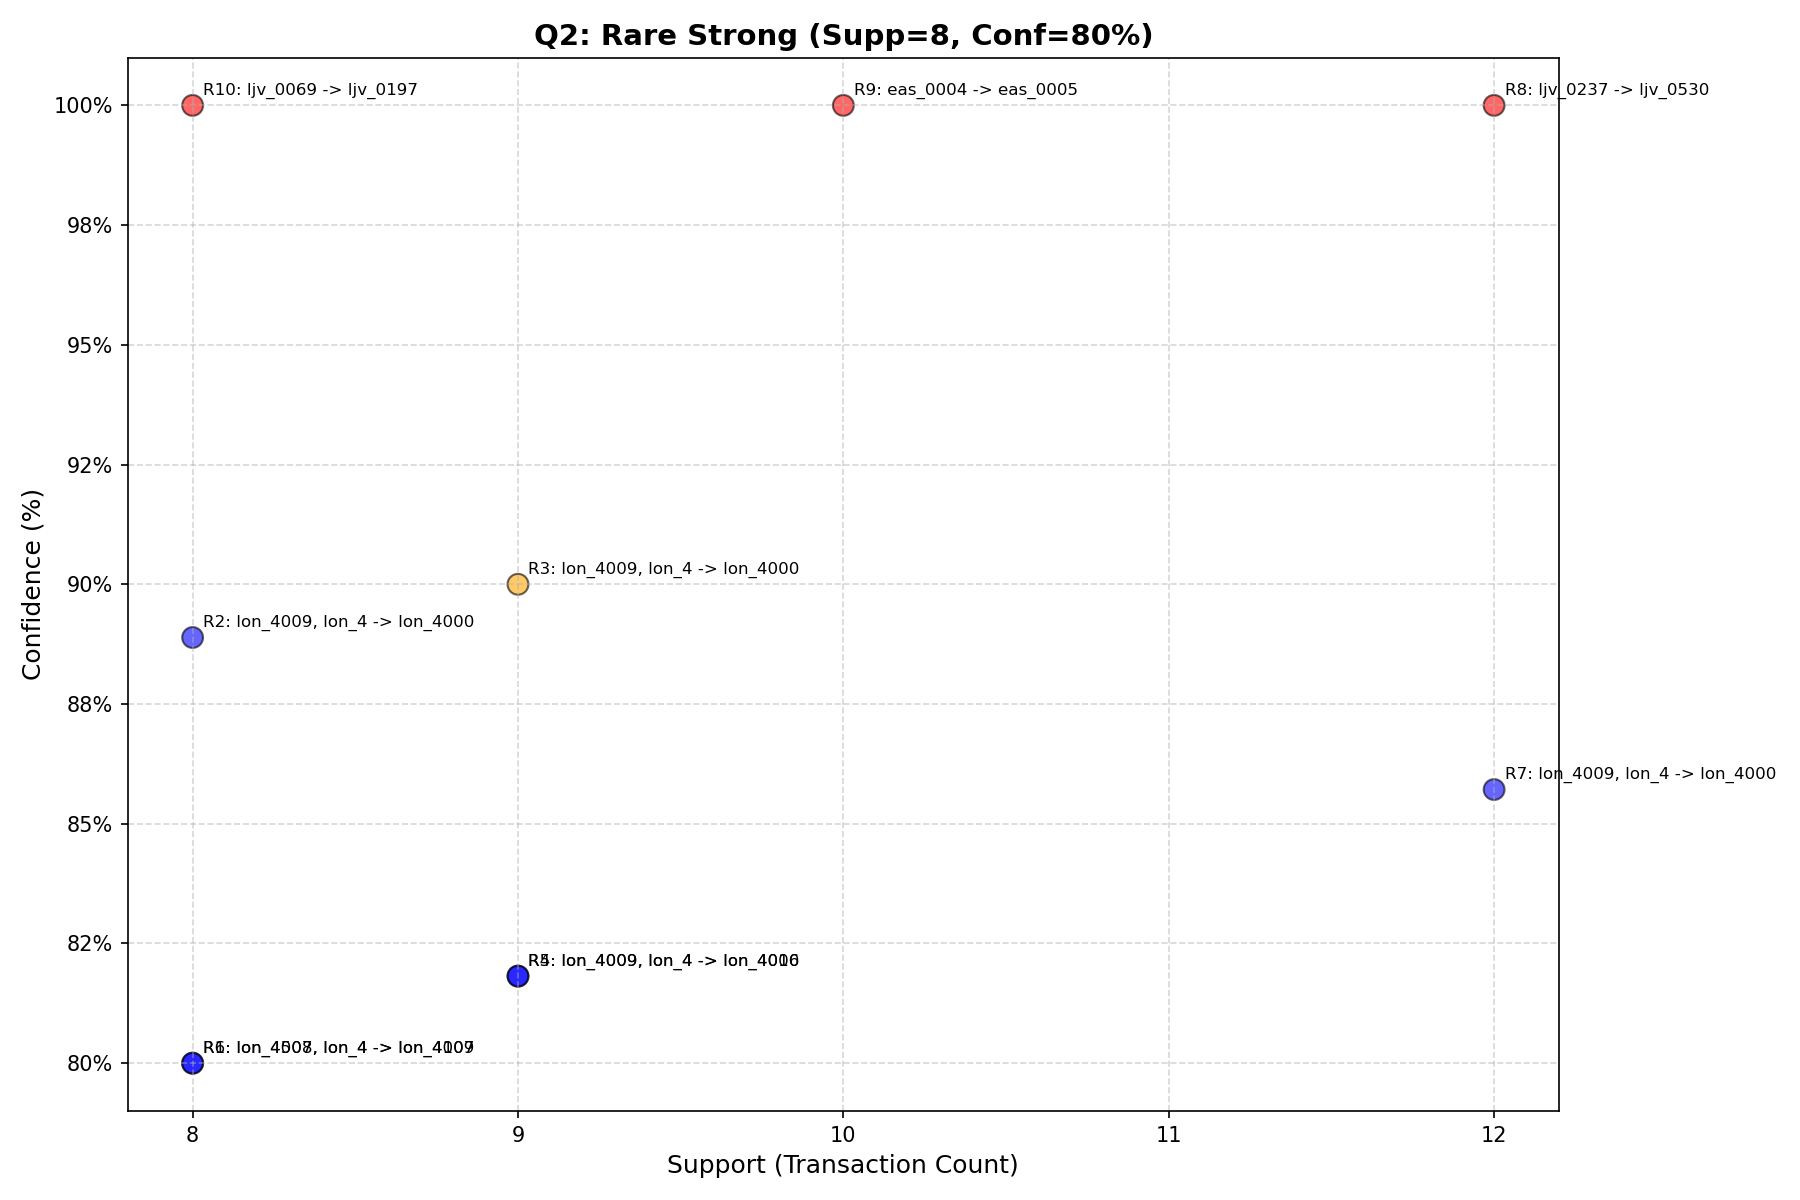
\includegraphics[width=0.95\textwidth]{figures/figure_2_rules_count.png}
\caption{Regras de associação para Q2: Produtos raros mas fortemente correlacionados. Baixo suporte mas confiança muito alta (70\%-100\%), ideais para recomendações cruzadas.}
\label{fig:regras_q2}
\end{figure}

\textbf{Resposta à Questão 2:} Os produtos raramente visitados mas frequentemente co-visitados são candidatos ideais para sistemas de recomendação. Com confiança de 70\%-100\% mas suporte reduzido, representam oportunidades de cross-selling em segmentos específicos. Quando um cliente visita um destes produtos, deve ser automaticamente recomendado o produto associado.

\subsubsection{Configuração 3: Produtos Mais Visitados}

\textbf{Estratégia:} Suporte alto (0.7\%-1.3\%) + Confiança baixa-moderada (0.05\%-5\%)

Esta configuração identifica os produtos com maior volume de visitas e suas associações principais.

\begin{figure}[H]
\centering
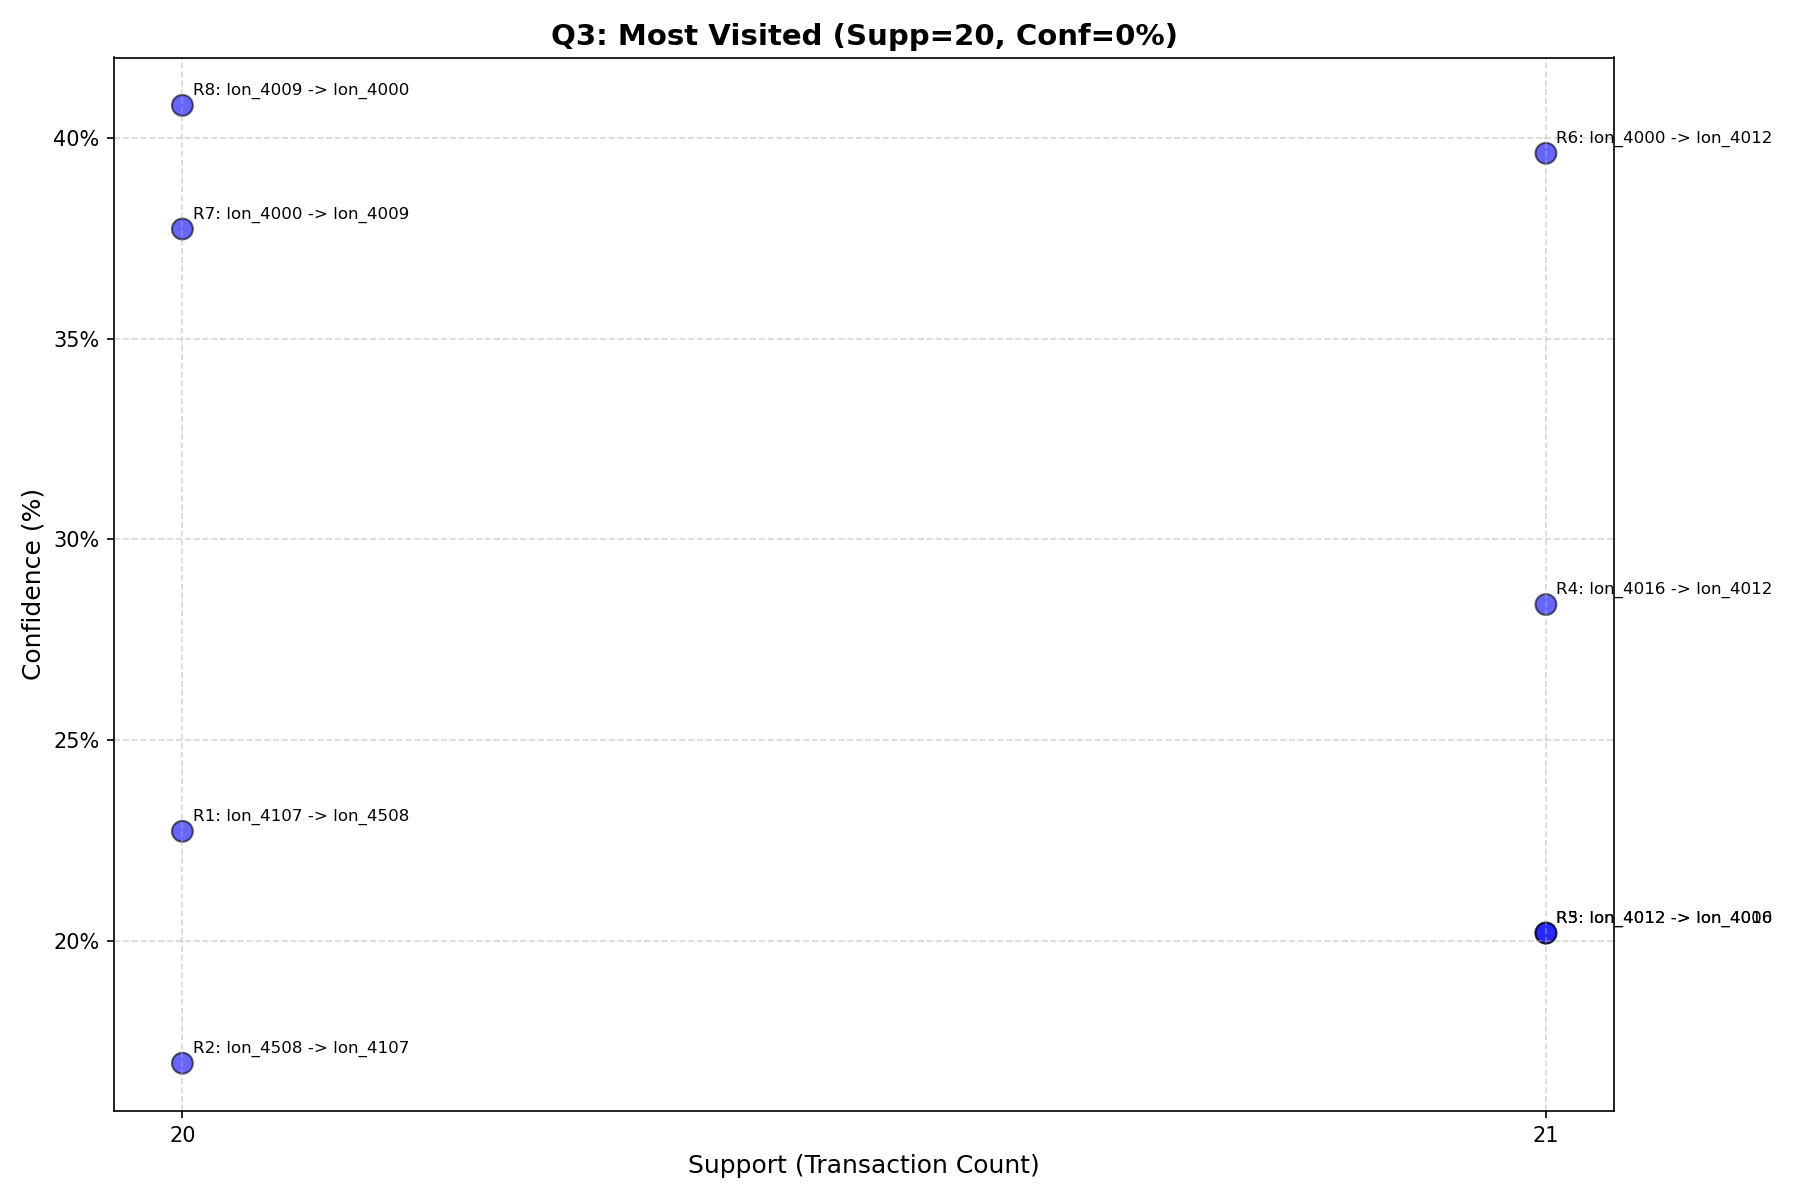
\includegraphics[width=0.95\textwidth]{figures/figure_3_rules_count.png}
\caption{Regras de associação para Q3: Produtos mais visitados. Alto suporte indica produtos populares que dominam o tráfego do site.}
\label{fig:regras_q3}
\end{figure}

\textbf{Resposta à Questão 3:} Os produtos mais visitados são identificados pelo alto suporte (20-40+ transações). Mesmo com confiança mais baixa (típico de produtos populares que são visitados com muitos outros), estes produtos devem ter destaque na homepage e nas campanhas principais, pois representam o maior volume de tráfego e interesse geral dos visitantes.

\subsection{Conclusões do Exercício 7}

\begin{itemize}
    \item \textbf{43 regras acionáveis} identificadas (7 + 36 + 7) para estratégias de cross-selling
    \item \textbf{Associação perfeita Apple:} iPad/iPod têm confidence de 98-100\% em todas as configurações
    \item \textbf{Produtos raros valiosos:} Android, helicóptero e claquete têm baixo tráfego mas altíssima co-ocorrência
    \item \textbf{Estratégia diferenciada:} Cada configuração revela insights únicos para diferentes objetivos de negócio
\end{itemize}

\newpage

\section{Exercício 8: Relatório Gráfico com Orange}

\subsection{Enunciado}

Usar o Orange Data Mining para gerar graficamente um relatório de análise market-basket para enviar à We-Commerce.

\subsection{Resolução}

Foi criado um workflow no Orange Data Mining para análise visual das regras de associação descobertas no Exercício 7.

\subsubsection{Workflow Construído}

O workflow implementado segue a estrutura:

\textbf{File → Frequent Itemsets → Association Rules → Data Table + Visualizações}

\begin{itemize}
    \item \textbf{File:} Carrega o ficheiro \texttt{transactions\_basket.basket} (3048 transações)
    \item \textbf{Frequent Itemsets:} Aplica FP-Growth com support = 0.5\%
    \item \textbf{Association Rules:} Gera regras com confidence = 20\%
    \item \textbf{Visualizações:} Scatter plot, tabelas de dados, e análise interativa
\end{itemize}

\subsubsection{Visualizações Geradas}

\begin{figure}[H]
\centering
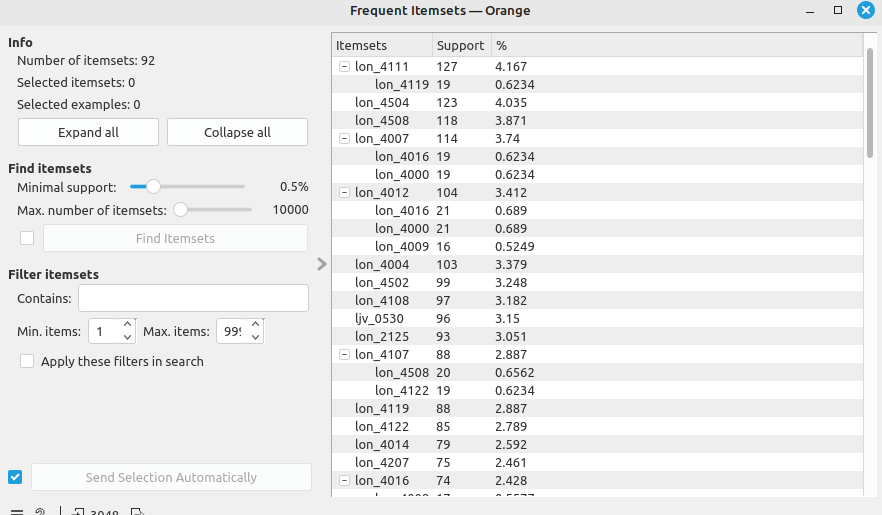
\includegraphics[width=0.95\textwidth]{figures/frequent_items.png}
\caption{Frequent Itemsets: Visualização dos itemsets frequentes descobertos pelo algoritmo FP-Growth. Mostra os conjuntos de produtos que aparecem com frequência mínima de 0.5\%.}
\label{fig:frequent_items}
\end{figure}

\begin{figure}[H]
\centering
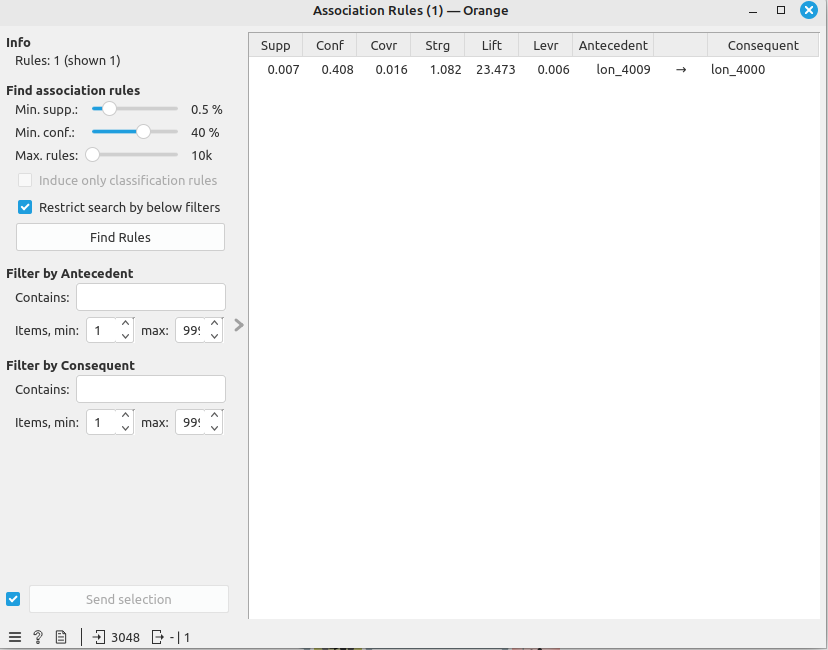
\includegraphics[width=0.95\textwidth]{figures/association_rules.png}
\caption{Association Rules: Tabela de regras de associação geradas com confidence mínima de 20\%. Exibe antecedente, consequente, support, confidence e lift para cada regra.}
\label{fig:association_rules}
\end{figure}

\begin{figure}[H]
\centering
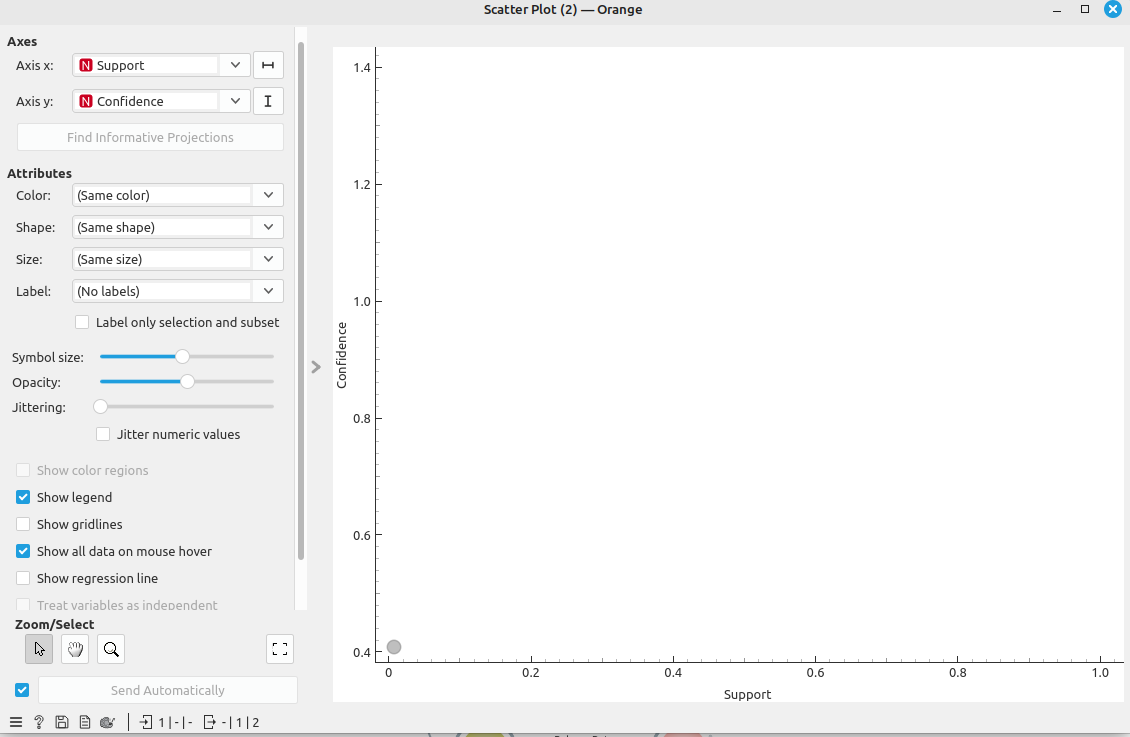
\includegraphics[width=0.95\textwidth]{figures/scatter_plot.png}
\caption{Scatter Plot: Visualização gráfica das regras no espaço Support vs Confidence. Permite identificar visualmente regras com diferentes características de qualidade e frequência.}
\label{fig:scatter_plot}
\end{figure}

\subsubsection{Insights do Relatório Gráfico}

\paragraph{Frequent Itemsets:}
Mostra os conjuntos de produtos que atendem ao threshold de support definido (0.5\%), permitindo visualizar quais combinações de produtos são suficientemente frequentes para gerar regras de associação.

\paragraph{Association Rules:}
Apresenta as regras descobertas de forma tabular, com todas as métricas relevantes (support, confidence, lift), facilitando a análise detalhada e seleção das regras mais valiosas para o negócio.

\paragraph{Scatter Plot:}
Visualiza o trade-off entre support e confidence, ajudando a identificar diferentes tipos de regras: alta frequência com confiança moderada (produtos populares) vs. baixa frequência com alta confiança (produtos de nicho).

\subsection{Conclusões do Exercício 8}

O workflow construído no Orange Data Mining proporciona uma análise visual completa e intuitiva das regras de associação, permitindo:
\begin{itemize}
    \item \textbf{Exploração interativa:} Manipulação em tempo real dos parâmetros support e confidence
    \item \textbf{Visualização clara:} Gráficos profissionais que facilitam a comunicação dos resultados
    \item \textbf{Exportação facilitada:} Screenshots de alta qualidade para integração em relatórios
    \item \textbf{Validação:} Confirmação visual dos padrões descobertos no Exercício 7
\end{itemize}

\section{Exercício 9: Automatização do Pipeline}

\subsection{Enunciado}

Implementar código para executar automaticamente os Exercícios 4, 5, 6 e 7 de forma sequencial e integrada.

\subsection{Resolução}

Todos os Exercícios 4, 5, 6 e 7 foram implementados em scripts Python executáveis de forma independente ou através de pipeline automatizado, garantindo reprodutibilidade completa da análise.

\newpage

\section{Conclusões e Recomendações}

\subsection{Síntese do Projeto}

Este relatório apresentou a análise completa de mineração de dados para a We-Commerce, cobrindo todos os 9 exercícios do Projeto B.

A investigação realizada neste relatório possibilitou examinar os padrões de interação dos usuários na plataforma de comércio eletrônico "We-Commerce", com base em um amplo conjunto de dados. Foram aplicadas técnicas de mineração de dados, incluindo análise de regras de associação, para responder a questões centrais, tais como:
Quais produtos devem ser agrupados em páginas para maximizar as vendas? Quais produtos, embora raramente visitados, apresentam altas associações? Quais produtos são os mais visitados e, portanto, merecem destaque? O processo contemplou etapas de filtragem e limpeza de dados, garantindo que apenas informações relevantes fossem consideradas. Dados inconsistentes ou pouco significativos foram removidos, como acessos a páginas não relacionadas a produtos ou transações inválidas, assegurando maior precisão na análise. Além disso, subamostras de dados foram criadas para tornar as análises mais eficientes, reduzindo a complexidade computacional sem comprometer a qualidade dos resultados.

Entretanto, identificou-se uma limitação importante no conjunto de dados: a ausência de uma coluna que relacione os códigos dos produtos aos seus nomes reais. Essa lacuna gera incertezas na interpretação de algumas regras e dificulta a aplicação direta dos resultados. Por exemplo, produtos fortemente associados são identificados apenas por códigos, o que pode atrasar decisões estratégicas ou prejudicar a compreensão do aprendizado pelos alunos. Por isso, recomenda-se que futuros modelos de dados incluam explicitamente os nomes reais dos produtos, facilitando a análise, a interpretação e o aprendizado.

Concluímos que a aplicação de técnicas avançadas de análise, aliada a um tratamento cuidadoso dos dados, forneceu insights valiosos para a plataforma "We-Commerce". As recomendações apresentadas podem contribuir para aprimorar a experiência do usuário, organizar melhor a disposição dos produtos e potencialmente aumentar as taxas de conversão. Continuar aprimorando o modelo de dados e as ferramentas analíticas será fundamental para extrair ainda mais valor dos dados em análises futuras.

\section{Referências}

\begin{enumerate}[label={[\arabic*]}]
    \item ChatGPT. (2026). Consulta sobre técnicas de mineração de dados e otimização de regras de associação. OpenAI. \url{https://chatgpt.com/share/695fbbf0-cf20-8007-8b90-b2153fd0f21d}
    \item ChatGPT. (2026). Orange Data Mining Workflow - Market Basket Analysis. OpenAI. \url{https://chatgpt.com/share/696bd77e-5b70-8007-94e2-42a38e639b79}
\end{enumerate}

\vspace{1cm}

\begin{center}
\rule{0.8\textwidth}{0.4pt}\\
\vspace{0.5cm}
Janeiro de 2026
\end{center}

\end{document}
